\documentclass[11pt,a4paper]{article}

\usepackage[utf8]{inputenc}
\usepackage[T1]{fontenc}
\usepackage[spanish,es-tabla]{babel}
\usepackage[margin=2.35cm]{geometry}
\usepackage{amsmath}
\usepackage{amssymb}
\usepackage{graphicx}
\usepackage{booktabs}
\usepackage{array}
\usepackage{float}
\usepackage{xcolor}
\usepackage{colortbl}
\definecolor{bestrow}{RGB}{220,245,220}
\usepackage{microtype}
\usepackage{hyperref}
\usepackage{listings}
\usepackage{enumitem}
\usepackage{caption}

\microtypesetup{expansion=false}

\hypersetup{
    colorlinks=true,
    linkcolor=blue!60!black,
    citecolor=blue!60!black,
    urlcolor=blue!60!black
}

\graphicspath{{artifacts/figures/generated/}{artifacts/figures/}}

\lstdefinestyle{codestyle}{
    basicstyle=\ttfamily\small,
    breaklines=true,
    frame=single,
    columns=fullflexible,
    keepspaces=true,
    showstringspaces=false,
    tabsize=2,
    backgroundcolor=\color{gray!5}
}

\lstset{style=codestyle}

\title{\textbf{Sistema de apoyo al análisis inicial de casos ante el TEDH (Tribunal Europeo de Derechos Humanos)}\\
\large Recuperación de precedentes, clasificación multietiqueta explicable y análisis de cambio entre particiones}

\author{
    Mauro Valls Vidal\\
    Alejandro Parra Sanchez\\
    Jordi Blasco Lozano\\
    Alejandro Martínez Riquelme\\[0.4em]
    \small Grado en Ingeniería en Inteligencia Artificial\\
    \small Escuela Politécnica Superior, Universidad de Alicante\\
    \small Aprendizaje Avanzado
}

\date{Curso 2025--2026}

\begin{document}

\maketitle

\begin{abstract}
Este trabajo presenta un sistema de apoyo al análisis inicial de casos ante el Tribunal Europeo de Derechos Humanos. A partir del texto de los hechos, el sistema sugiere artículos candidatos del Convenio Europeo de Derechos Humanos, recupera precedentes similares y ofrece señales de auditoría sobre las predicciones. El proyecto utiliza LexGLUE ECtHR Task B, con 11000 casos, diez artículos posibles y 15991 pares positivos entre caso y artículo. La solución combina clasificación multietiqueta, TF-IDF dentro de \texttt{Pipeline}, clasificadores One-vs-Rest, recuperación por similitud coseno y explicaciones con coeficientes y LIME. Los hiperparámetros se seleccionan con \texttt{GridSearchCV} y validación cruzada de 5 folds usando solo train. Después, el mejor estimador se reentrena con todo train y test queda reservado para la evaluación final. En test, la SVM lineal obtiene el mejor rendimiento, con macro-F1 de 0.749, micro-F1 de 0.777 y Hamming loss de 0.061. La regresión logística queda cerca, con macro-F1 de 0.736, y se mantiene como modelo auditado por sus coeficientes interpretables. En recuperación de precedentes, TF-IDF con coseno alcanza Recall@10 de 0.972 en test. El sistema no sustituye el criterio jurídico. Su valor está en priorizar hipótesis revisables y facilitar una auditoría inicial.
\end{abstract}

\noindent\textbf{Palabras clave}
NLP jurídico, ECtHR, LexGLUE, clasificación multietiqueta, TF-IDF, One-vs-Rest, explicabilidad, LIME, retrieval, drift.

\tableofcontents
\newpage

\section{Introducción}
\label{sec_intro}

El análisis de un caso ante el Tribunal Europeo de Derechos Humanos exige leer hechos extensos, detectar artículos potencialmente implicados y revisar jurisprudencia relacionada. Esta tarea consume tiempo y requiere atención técnica. Un error en esta fase inicial puede tener consecuencias prácticas. Si se omite un artículo relevante, se puede perder una línea de argumentación. Si se revisan demasiados artículos irrelevantes, aumenta la carga de trabajo y se dispersa el análisis.

El proyecto aborda este escenario con aprendizaje automático. El sistema recibe como entrada el texto de un caso y devuelve una salida pensada para ser revisada por una persona. La salida no es una decisión judicial. Tampoco es una predicción de culpabilidad, responsabilidad o resultado procesal. La salida es una propuesta de apoyo formada por artículos candidatos, casos similares y señales explicables.

La idea principal es convertir un conjunto de documentos jurídicos largos en una estructura de datos útil. Primero se descarga y normaliza el dataset LexGLUE ECtHR Task B. Después se guarda en una base SQLite con tablas separadas para casos, párrafos, artículos y etiquetas. A partir de esa base se construyen matrices de aprendizaje automático. El texto se representa con TF-IDF y la salida se modela como clasificación multietiqueta. Cada artículo se trata como una etiqueta binaria independiente dentro de una estrategia One-vs-Rest.

El trabajo se ha diseñado con tres prioridades. La primera es la reproducibilidad. Todas las fases están separadas en notebooks numerados y usan funciones comunes en un archivo Python. La segunda es la interpretabilidad. Se usan modelos lineales y explicaciones locales para que el comportamiento pueda auditarse. La tercera es la discusión crítica. El proyecto no se limita a reportar métricas, sino que analiza falsos positivos, falsos negativos, cambio entre particiones y riesgos de despliegue.

La memoria está organizada de forma progresiva. Primero se presenta el contexto y el trabajo relacionado. Después se describe el dataset y la formulación del problema. A continuación se explica la organización del código, la metodología, los experimentos y los resultados. Finalmente se discuten limitaciones, riesgos y posibles mejoras.

\section{Contexto y trabajo relacionado}
\label{sec_contexto}

\subsection{NLP jurídico y LexGLUE}

El procesamiento de lenguaje natural jurídico busca aplicar técnicas de aprendizaje automático a textos legales. Estos textos tienen rasgos particulares. Suelen ser largos, técnicos, densos y dependientes de contexto. Además, los errores pueden tener impacto social, económico o legal. Por eso no basta con entrenar un modelo y medir una métrica global. Es necesario explicar qué tarea se resuelve, qué límites tiene el sistema y cómo debe usarse.

LexGLUE es un benchmark de comprensión de lenguaje jurídico en inglés. Incluye varias tareas y una de ellas se basa en casos del Tribunal Europeo de Derechos Humanos. En este proyecto se utiliza ECtHR Task B. La tarea consiste en identificar artículos del Convenio Europeo de Derechos Humanos asociados a los hechos de un caso. Esto convierte el problema en clasificación multietiqueta, porque un caso puede estar relacionado con más de un artículo.

La elección de LexGLUE tiene varias ventajas. El dataset es público, está dividido en particiones oficiales y permite comparar resultados de forma reproducible. También permite trabajar con un dominio real y complejo sin tratar expedientes privados. Aun así, su uso requiere cuidado. El hecho de que un modelo acierte artículos no significa que razone jurídicamente. El sistema identifica patrones textuales asociados a etiquetas, no interpreta normas como lo haría un jurista.

\subsection{Predicción jurídica y alcance responsable}

La literatura sobre predicción jurídica ha mostrado que los textos de casos contienen señales útiles para anticipar resultados o categorías legales. Sin embargo, este tipo de trabajo puede inducir interpretaciones exageradas. Un modelo puede aprender correlaciones presentes en los datos sin comprender el razonamiento jurídico subyacente.

Por esta razón, este proyecto evita presentar el sistema como un juez automático. El encuadre correcto es más limitado y más responsable. El sistema ayuda en una fase inicial de análisis. Su función es sugerir qué artículos revisar y qué casos anteriores podrían ser útiles. La decisión final, la interpretación jurídica y la valoración normativa quedan fuera del modelo.

\subsection{Explicabilidad y auditoría}

La explicabilidad es especialmente importante en derecho. Si un sistema sugiere un artículo, el usuario necesita saber qué señales textuales influyeron en esa sugerencia. En este proyecto se combinan dos niveles de explicación.

El primer nivel es global. Para cada artículo se inspeccionan los coeficientes del modelo lineal. Esto permite ver qué términos empujan una predicción hacia una etiqueta concreta. El segundo nivel es local. Para algunos casos individuales se usa LIME, que aproxima el comportamiento del modelo alrededor de una entrada y muestra términos relevantes para esa predicción.

Estas explicaciones no son pruebas jurídicas. Tampoco demuestran causalidad. Sirven para auditar el modelo y detectar señales razonables, señales espurias o posibles fuentes de error.

\subsection{Cambio entre particiones}

Los sistemas de aprendizaje automático pueden degradarse cuando cambia la distribución de los datos. En este trabajo se analiza el cambio entre train, validation y test. La versión usada del dataset no proporciona un año oficial de sentencia para todos los registros, por lo que no se afirma deriva temporal estricta. Se habla con más precisión de cambio entre particiones.

El análisis compara distribuciones de etiquetas y diferencias de rendimiento. Esto ayuda a responder una pregunta práctica. Si el modelo funciona bien en validación, cuánto cambia su comportamiento en test. Esta pregunta es clave para valorar robustez.

\section{Descripción del problema}
\label{sec_problema}

\subsection{Objetivo del sistema}

El objetivo es construir un sistema que, dado el texto de un caso del TEDH, produzca una ayuda estructurada para el análisis inicial. La salida esperada contiene tres elementos.

\begin{enumerate}[label=\arabic*.]
    \item Un conjunto de artículos candidatos del Convenio Europeo de Derechos Humanos.
    \item Una lista ordenada de casos previos similares que puedan servir como precedentes de revisión.
    \item Señales de explicación y auditoría sobre el comportamiento del modelo.
\end{enumerate}

El sistema no decide si hubo violación de derechos. Tampoco sustituye una lectura jurídica completa. Funciona como una herramienta de priorización.

\subsection{Formulación multietiqueta}

Cada caso se representa como un documento textual \(x_i\). La salida real es un vector binario \(y_i\) con diez posiciones. Cada posición representa un artículo. El valor uno indica que el artículo está asociado al caso. El valor cero indica que no aparece como etiqueta positiva.

\[
y_i \in \{0,1\}^{K}
\]

\[
K = 10
\]

El modelo aprende una función que asigna un score o una decisión a cada artículo.

\[
f(x_i) \rightarrow \hat{y}_i \in \{0,1\}^{K}
\]

Este diseño es necesario porque el problema no es multiclase. En clasificación multiclase cada ejemplo pertenece a una única clase. Aquí un caso puede implicar varios artículos al mismo tiempo. Por eso se necesita una matriz de etiquetas y métricas multietiqueta.

\subsection{Consecuencias de los errores}

No todos los errores tienen la misma interpretación. Un falso positivo ocurre cuando el sistema sugiere un artículo que no aparece como etiqueta real. En la práctica, esto puede añadir trabajo de revisión y ruido. Un falso negativo ocurre cuando el sistema no sugiere un artículo que sí era relevante. Este error puede ser más grave porque puede ocultar una línea de análisis.

Esta diferencia justifica estudiar patrones de error además de métricas agregadas. Una puntuación global puede parecer aceptable y aun así esconder muchos falsos negativos en etiquetas minoritarias.

\section{Datos utilizados}
\label{sec_datos}

\subsection{Origen y contenido}

El dataset utilizado es LexGLUE ECtHR Task B. Contiene casos del Tribunal Europeo de Derechos Humanos y etiquetas asociadas a artículos del Convenio. La entrada principal es el texto de los hechos. La salida son artículos jurídicos representados como etiquetas.

La Tabla \ref{tab_dataset} resume el tamaño del dataset usado tras la ingesta.

\begin{table}[H]
\centering
\caption{Características principales del dataset}
\label{tab_dataset}
\small
\begin{tabular}{@{}lr@{}}
\toprule
\textbf{Elemento} & \textbf{Valor}\\
\midrule
Casos de entrenamiento & 9000\\
Casos de validación & 1000\\
Casos de test & 1000\\
Casos totales & 11000\\
Artículos posibles & 10\\
Pares positivos caso artículo & 15991\\
Media de artículos por caso etiquetado & 1.477\\
Máximo de artículos en un caso & 7\\
Párrafos almacenados & 262580\\
\bottomrule
\end{tabular}
\end{table}

Los artículos considerados son 2, 3, 5, 6, 8, 9, 10, 11, 14 y P1-1. Algunos son frecuentes y otros aparecen mucho menos. Este desbalance condiciona la evaluación y justifica usar macro-F1 como métrica principal de selección.

\subsection{Particiones oficiales}

El dataset ya viene dividido en train, validation y test. El proyecto respeta esa división. Train se usa para seleccionar hiperparámetros con \texttt{GridSearchCV} y validación cruzada de 5 folds. El mejor estimador se reentrena con todo train. Validation queda como split informativo. Test se reserva para la evaluación final.

Esta separación evita fuga de información. Si el vectorizador, los hiperparámetros o la arquitectura se ajustaran con test, los resultados finales serían demasiado optimistas.

\subsection{Análisis exploratorio}

El EDA resume los rasgos principales del dataset usado en el proyecto. La partición oficial contiene 9000 casos de train, 1000 de validation y 1000 de test. Los textos son largos y variables, con documentos entre 70 y 35780 tokens. Las etiquetas están desbalanceadas. El artículo 6 aparece en 6225 casos, mientras que el artículo 9 aparece en 101. Además, la tarea es multietiqueta. La media es de 1.477 artículos por caso etiquetado y el máximo observado es de 7 artículos.

\begin{figure}[H]
\centering
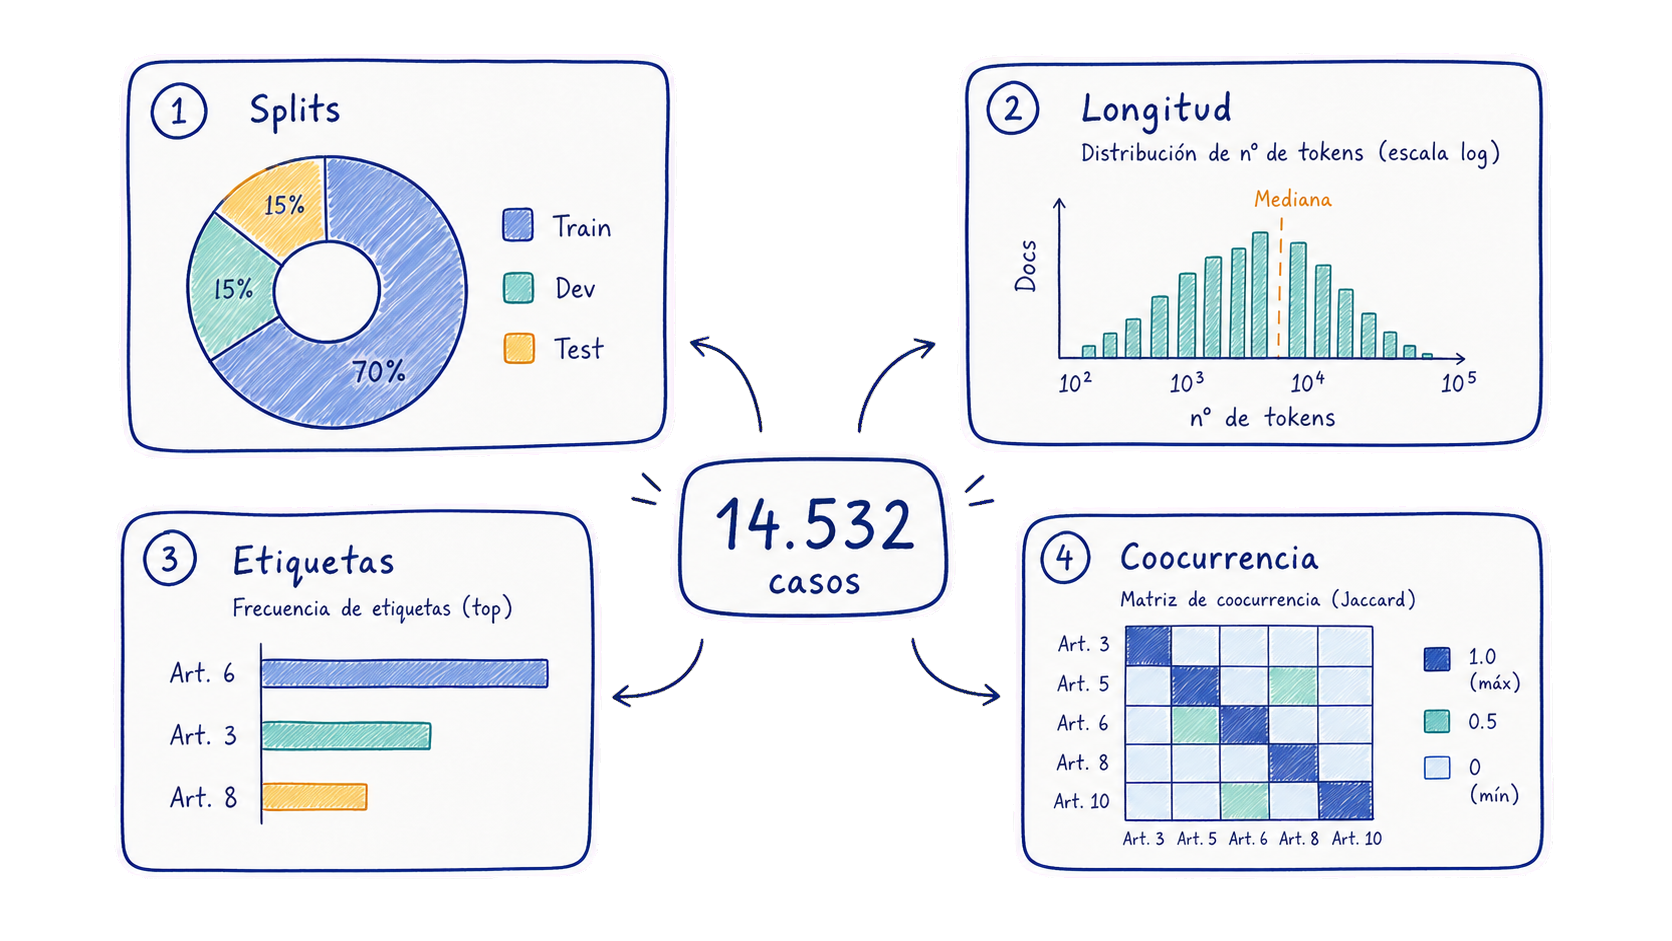
\includegraphics[width=0.92\textwidth]{notebook_01_eda_v2.png}
\caption{Frecuencia de artículos y cardinalidad multietiqueta}
\label{fig_eda}
\end{figure}

Estos resultados justifican varias decisiones. El uso de TF-IDF permite manejar textos largos de forma eficiente. La formulación One-vs-Rest permite predecir varios artículos por caso. El uso de macro-F1 permite observar mejor el rendimiento en etiquetas minoritarias. El desbalanceo también justifica probar pesos de clase cuando el modelo lo permite.

No se reduce la etiqueta mayoritaria eliminando casos del artículo 6 como decisión principal. El problema es multietiqueta, no multiclase. Si se eliminan casos con artículo 6, también se eliminan positivos de otros artículos que aparecen en esos mismos casos. Por eso se conservan los splits oficiales, se prueban pesos de clase cuando procede y se evalúa con macro-F1.

\section{Organización del proyecto}
\label{sec_organizacion}

\subsection{Estructura general}

El proyecto está organizado alrededor de seis notebooks, un módulo común, un esquema SQL, documentación y artefactos. La estructura principal es la siguiente.

\begin{lstlisting}[language=bash]
proyecto final
  README.md
  explicacion.md
  requirements.txt
  schema.sql
  project_utils.py
  00_ingesta_y_esquema_relacional.ipynb
  01_EDA.ipynb
  02_modelado_multilabel.ipynb
  03_retrieval_de_precedentes.ipynb
  04_xai_drift_y_errores.ipynb
  05_guion_informe_y_defensa.ipynb
  artifacts
    figures
    indices
\end{lstlisting}

Los notebooks implementan el flujo experimental. El archivo \texttt{project\_utils.py} contiene funciones compartidas. El archivo \texttt{schema.sql} define la base de datos. La carpeta \texttt{artifacts} guarda salidas, figuras e índices.

\subsection{Papel de cada notebook}

El notebook \texttt{00\_ingesta\_y\_esquema\_relacional.ipynb} prepara la base de datos. Carga LexGLUE, normaliza párrafos, crea identificadores de caso y guarda casos, párrafos, artículos y etiquetas en SQLite.

El notebook \texttt{01\_EDA.ipynb} analiza la calidad y distribución de los datos. Calcula tamaños por split, estadísticas de longitud, frecuencia de artículos, densidad multietiqueta y coocurrencias.

El notebook \texttt{02\_modelado\_multilabel.ipynb} entrena y evalúa los modelos. Construye textos y etiquetas, define pipelines completos con TF-IDF, selecciona hiperparámetros con \texttt{GridSearchCV}, compara modelos y guarda predicciones.

El notebook \texttt{03\_retrieval\_de\_precedentes.ipynb} implementa la búsqueda de precedentes. Construye índices TF-IDF y TF-IDF con SVD. Evalúa rankings con Recall@k y nDCG@10.

El notebook \texttt{04\_xai\_drift\_y\_errores.ipynb} audita el sistema. Extrae términos globales, genera explicaciones locales con LIME, calcula cambio entre particiones y estudia falsos positivos y falsos negativos.

El notebook \texttt{05\_guion\_informe\_y\_defensa.ipynb} consolida evidencias para la memoria y la defensa. Comprueba artefactos esperados y relaciona resultados con la rúbrica.

\subsection{Módulo común}

El archivo \texttt{project\_utils.py} evita duplicación. Define rutas, constantes, códigos de artículos, funciones de base de datos, carga de datos, construcción de matrices y métricas.

Un ejemplo conceptual de la función que construye la matriz multietiqueta es el siguiente.

\begin{lstlisting}
FUNCION multilabel_matrix con labels, case_ids y articles
    crear una matriz Y llena de ceros
    usar una fila por caso
    usar una columna por articulo
    PARA CADA etiqueta positiva del dataset
        localizar su caso y su articulo
        escribir 1 en la celda correspondiente
    FIN
    devolver Y
\end{lstlisting}

Esta función es central porque transforma pares positivos caso artículo en una matriz binaria. Sin esta matriz no se podría entrenar un clasificador multietiqueta.

\subsection{Esquema SQLite}

El archivo \texttt{schema.sql} define una base relacional normalizada. Las tablas más importantes son las siguientes.

\begin{itemize}
    \item \texttt{cases} guarda un caso por fila con split, texto completo y metadatos de longitud.
    \item \texttt{case\_paragraphs} guarda los párrafos originales para mantener trazabilidad.
    \item \texttt{articles} contiene el catálogo de etiquetas.
    \item \texttt{case\_labels} contiene los pares positivos entre caso y artículo.
    \item \texttt{experiment\_runs} guarda información de cada ejecución.
    \item \texttt{predictions} guarda etiquetas reales, predicciones y scores.
    \item \texttt{explanations} guarda resúmenes o rutas de explicaciones.
\end{itemize}

Esta base permite que los notebooks compartan una misma fuente de verdad. También facilita auditoría porque cada predicción puede relacionarse con el caso y la ejecución que la generó.

\begin{figure}[H]
\centering
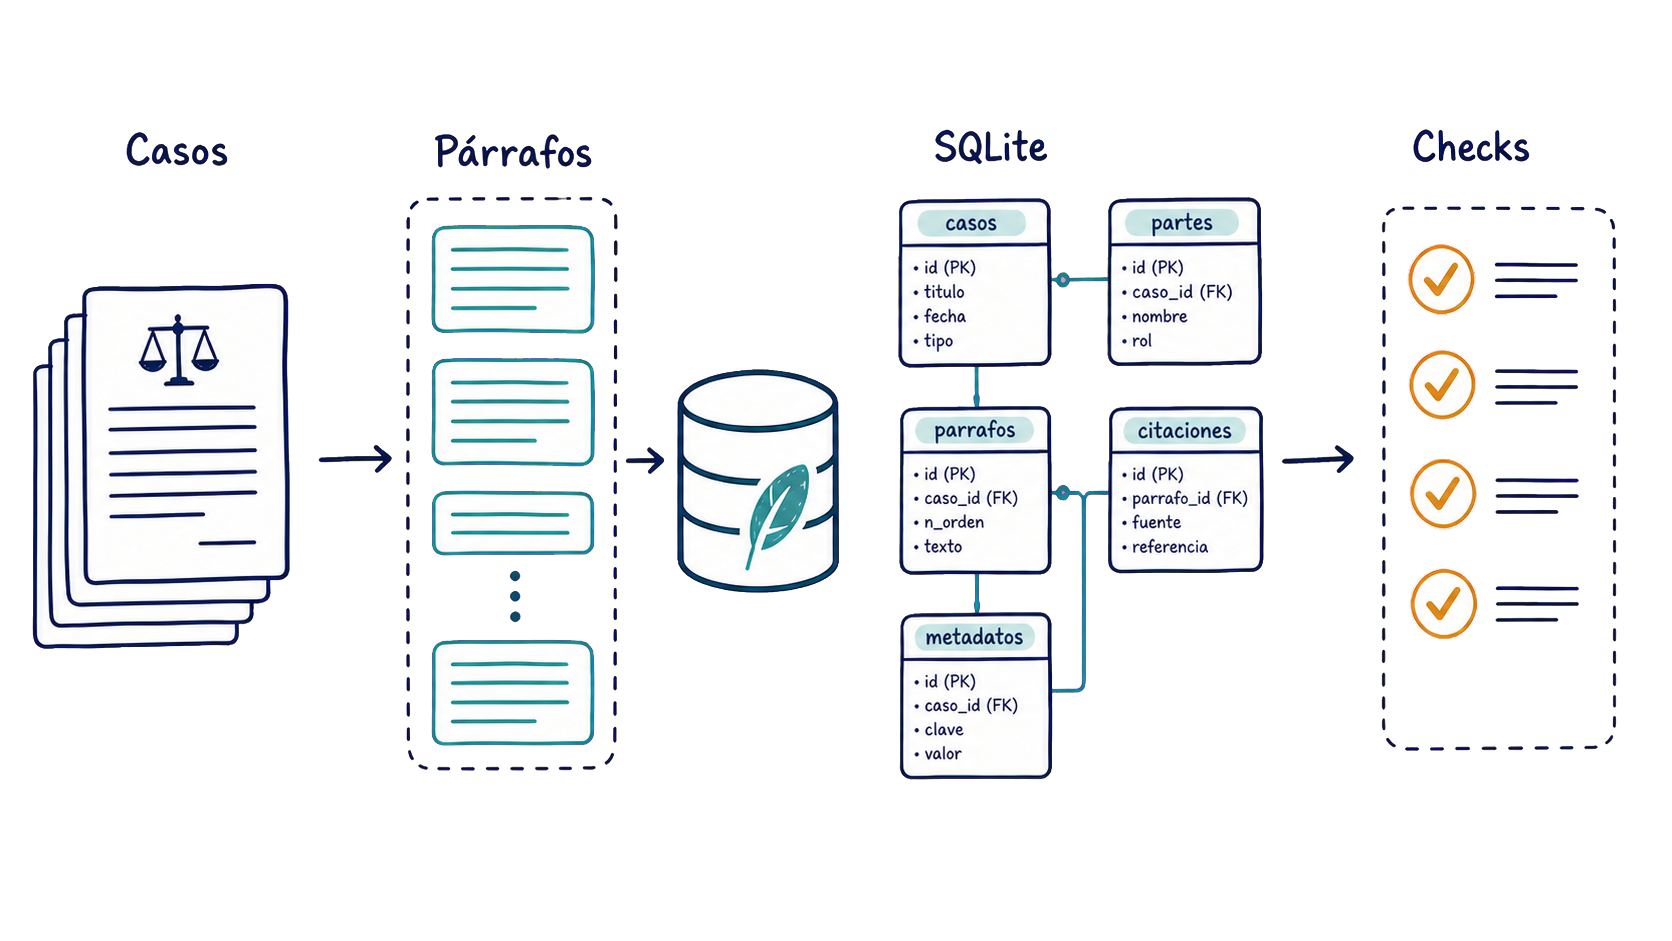
\includegraphics[width=0.92\textwidth]{notebook_00_ingestion_schema_v2.png}
\caption{Esquema conceptual de ingesta y almacenamiento}
\label{fig_schema}
\end{figure}

\section{Tecnologías utilizadas}
\label{sec_tecnologias}

El proyecto utiliza Python como lenguaje principal. Las librerías principales son \texttt{pandas} y \texttt{numpy} para manipulación de datos, \texttt{sqlite3} para almacenamiento, \texttt{datasets} para cargar LexGLUE, \texttt{scikit-learn} para vectorización, modelos y métricas, \texttt{joblib} para persistencia de artefactos, \texttt{matplotlib} y \texttt{seaborn} para visualización, y \texttt{lime} para explicabilidad local.

La elección de estas tecnologías responde a una idea simple. El proyecto debe ser reproducible, entendible y ejecutable en un entorno estándar. Por eso se priorizan herramientas ampliamente usadas y modelos que puedan inspeccionarse.

El archivo \texttt{requirements.txt} recoge las dependencias necesarias. Esto facilita crear un entorno limpio y ejecutar los notebooks en orden.

\section{Diseño de la solución}
\label{sec_diseno}

\subsection{Flujo completo}

El flujo interno puede entenderse como una cadena de transformaciones.

\begin{figure}[H]
\centering
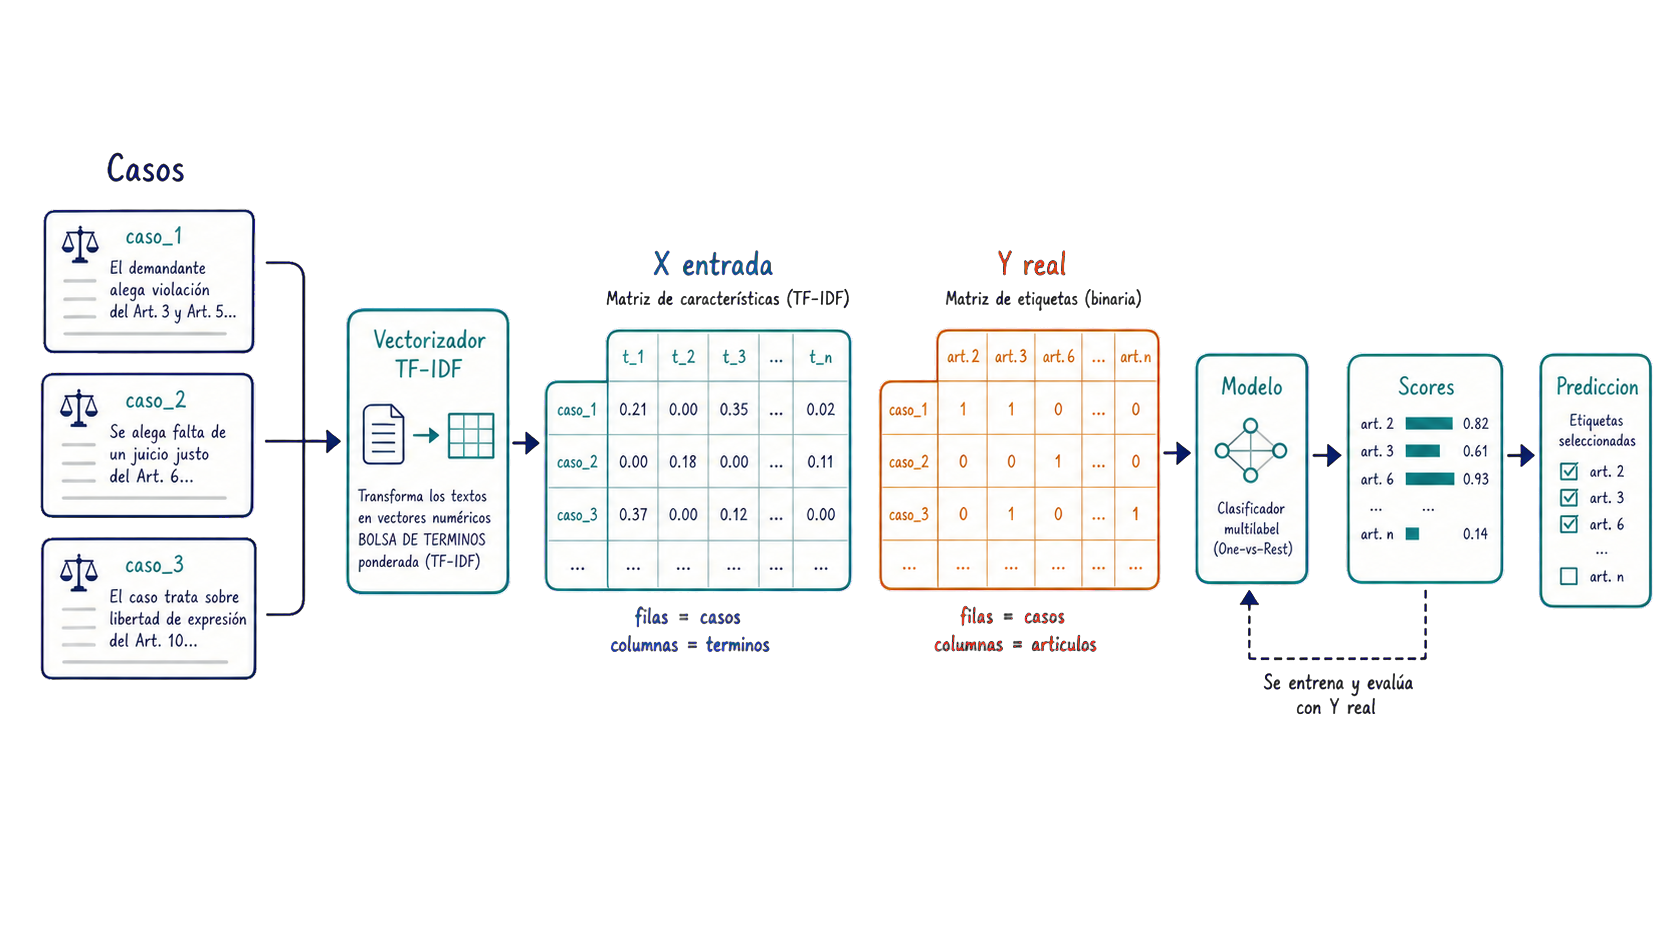
\includegraphics[width=0.92\textwidth]{notebook_02_xy_matrix_flow_v2.png}
\caption{Transformación desde textos y etiquetas hasta matrices de modelado}
\label{fig_xy}
\end{figure}

Primero, cada caso se convierte en texto completo mediante la unión de párrafos. Segundo, las etiquetas se convierten en columnas binarias. Tercero, se define un pipeline completo con TF-IDF y clasificador. Cuarto, se seleccionan hiperparámetros con \texttt{GridSearchCV} y 5 folds sobre train. Quinto, el mejor estimador se reentrena con todo train. Sexto, test se evalúa al final y las predicciones se guardan para auditoría.

\subsection{Representación TF-IDF}

TF-IDF representa un documento como un vector de términos ponderados. Un término recibe más peso si aparece con frecuencia en un documento y no aparece de forma excesiva en todos los documentos. Esto es útil en textos jurídicos porque ciertas palabras pueden ser muy indicativas de artículos concretos.

El vectorizador usa unigramas y bigramas. Los unigramas capturan palabras individuales. Los bigramas capturan expresiones de dos palabras, como \texttt{domestic violence} o \texttt{fair trial}. El tamaño del vocabulario se selecciona dentro de la búsqueda de hiperparámetros.

La configuración se incluye dentro de un \texttt{Pipeline}. Esto evita leakage durante la validación cruzada porque TF-IDF se ajusta de nuevo en cada fold usando solo la parte de entrenamiento del fold.

\begin{lstlisting}[language=Python]
TfidfVectorizer(
    ngram_range=(1, 2),
    max_df=0.95,
    sublinear_tf=True,
    strip_accents='unicode',
    lowercase=True
)
\end{lstlisting}

La búsqueda prueba distintos valores de \texttt{min\_df} y \texttt{max\_features}. Test no se usa para elegir esos valores.

\subsection{Clasificación One-vs-Rest}

La estrategia One-vs-Rest entrena un clasificador independiente por artículo. Para el artículo 2, el modelo aprende a distinguir casos que tienen ese artículo frente a casos que no lo tienen. Lo mismo se repite para los diez artículos.

Este diseño encaja bien con el problema. Permite que varias etiquetas sean positivas en el mismo caso. Además, con regresión logística se obtiene un score interpretable por etiqueta.

El flujo general de los modelos es el siguiente.

\begin{lstlisting}[language=Python]
Pipeline
    TfidfVectorizer
    clasificador One-vs-Rest
GridSearchCV con 5 folds sobre train
refit del mejor estimador con todo train
evaluación final en test
\end{lstlisting}

\subsection{Selección de hiperparámetros}

La selección de hiperparámetros se realiza con \texttt{GridSearchCV}. La búsqueda usa solo train y aplica validación cruzada de 5 folds. La métrica principal es macro-F1 porque da más peso a las etiquetas minoritarias.

Para regresión logística y SVM se prueban valores de \texttt{C}, \texttt{min\_df}, \texttt{max\_features} y \texttt{class\_weight}. Para la variante neuronal se usa TF-IDF, TruncatedSVD, escalado y MLP dentro del mismo pipeline. En ese caso se prueban el número de componentes SVD, el tamaño de la capa oculta y la regularización \texttt{alpha}.

El mejor estimador queda reentrenado con todo train mediante \texttt{refit=True}. Test solo se usa después para estimar el rendimiento final. No se ajustan umbrales, arquitectura ni hiperparámetros con test.

\begin{figure}[H]
\centering
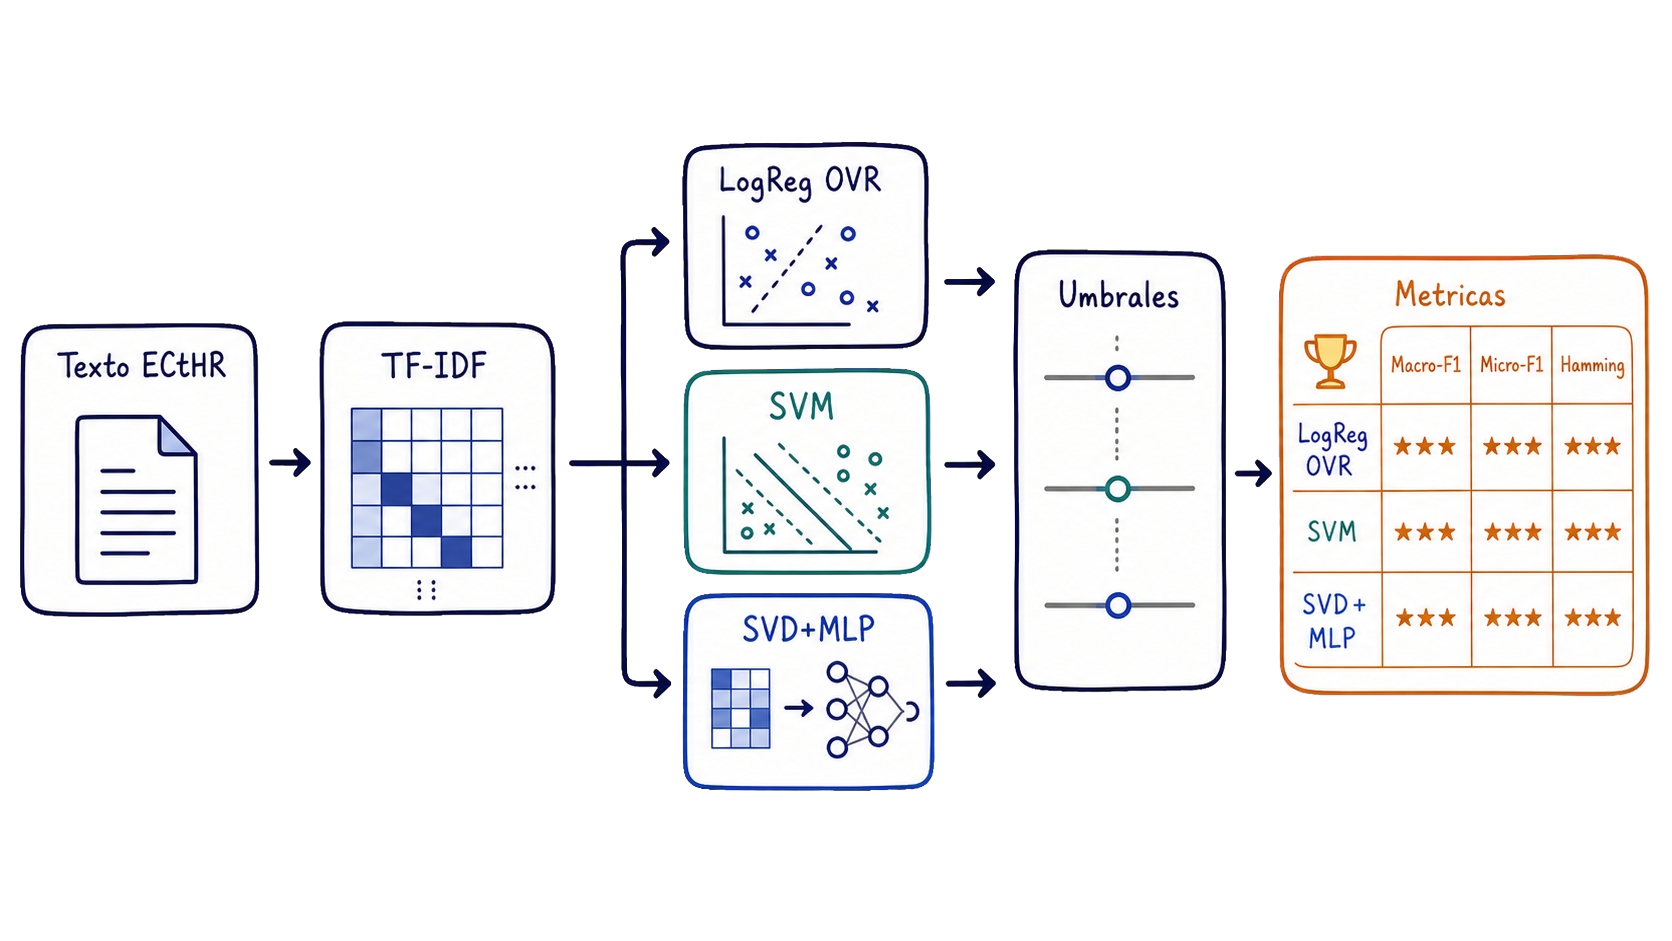
\includegraphics[width=0.92\textwidth]{notebook_02_modeling_v2.png}
\caption{Resumen visual del modelado multietiqueta}
\label{fig_modelado}
\end{figure}

\subsection{Comparación de modelos}

El notebook de modelado incluye varias referencias. Se usa un baseline de artículo frecuente, regresión logística One-vs-Rest, SVM lineal One-vs-Rest y una variante TF-IDF con SVD y MLP. Todos los modelos entrenables se ajustan con \texttt{GridSearchCV} sobre train. La comparativa final se reporta con test.

La SVM lineal obtiene mejores métricas en la evaluación final de test. Aun así, las explicaciones posteriores se apoyan en la regresión logística porque sus coeficientes se interpretan de forma directa. La variante MLP sirve como comparación no lineal adicional. No debe presentarse como núcleo del sistema porque no supera a los modelos lineales.

\section{Recuperación de precedentes}
\label{sec_retrieval}

\subsection{Motivación}

En análisis jurídico no basta con sugerir artículos. También es útil recuperar casos parecidos. Un precedente puede orientar la lectura, mostrar patrones de hechos y ayudar a comparar argumentos. Por eso el proyecto incluye un módulo de retrieval.

El sistema indexa una muestra de casos de entrenamiento. Después, para cada consulta de validation o test, calcula similitud coseno con los casos indexados y devuelve los más parecidos.

\subsection{Métodos evaluados}

Se evalúan dos métodos. El primero usa directamente los vectores TF-IDF y similitud coseno. El segundo aplica TruncatedSVD para reducir dimensión y después calcula coseno. SVD puede agrupar términos correlacionados en componentes latentes, aunque reduce interpretabilidad directa.

\begin{figure}[H]
\centering
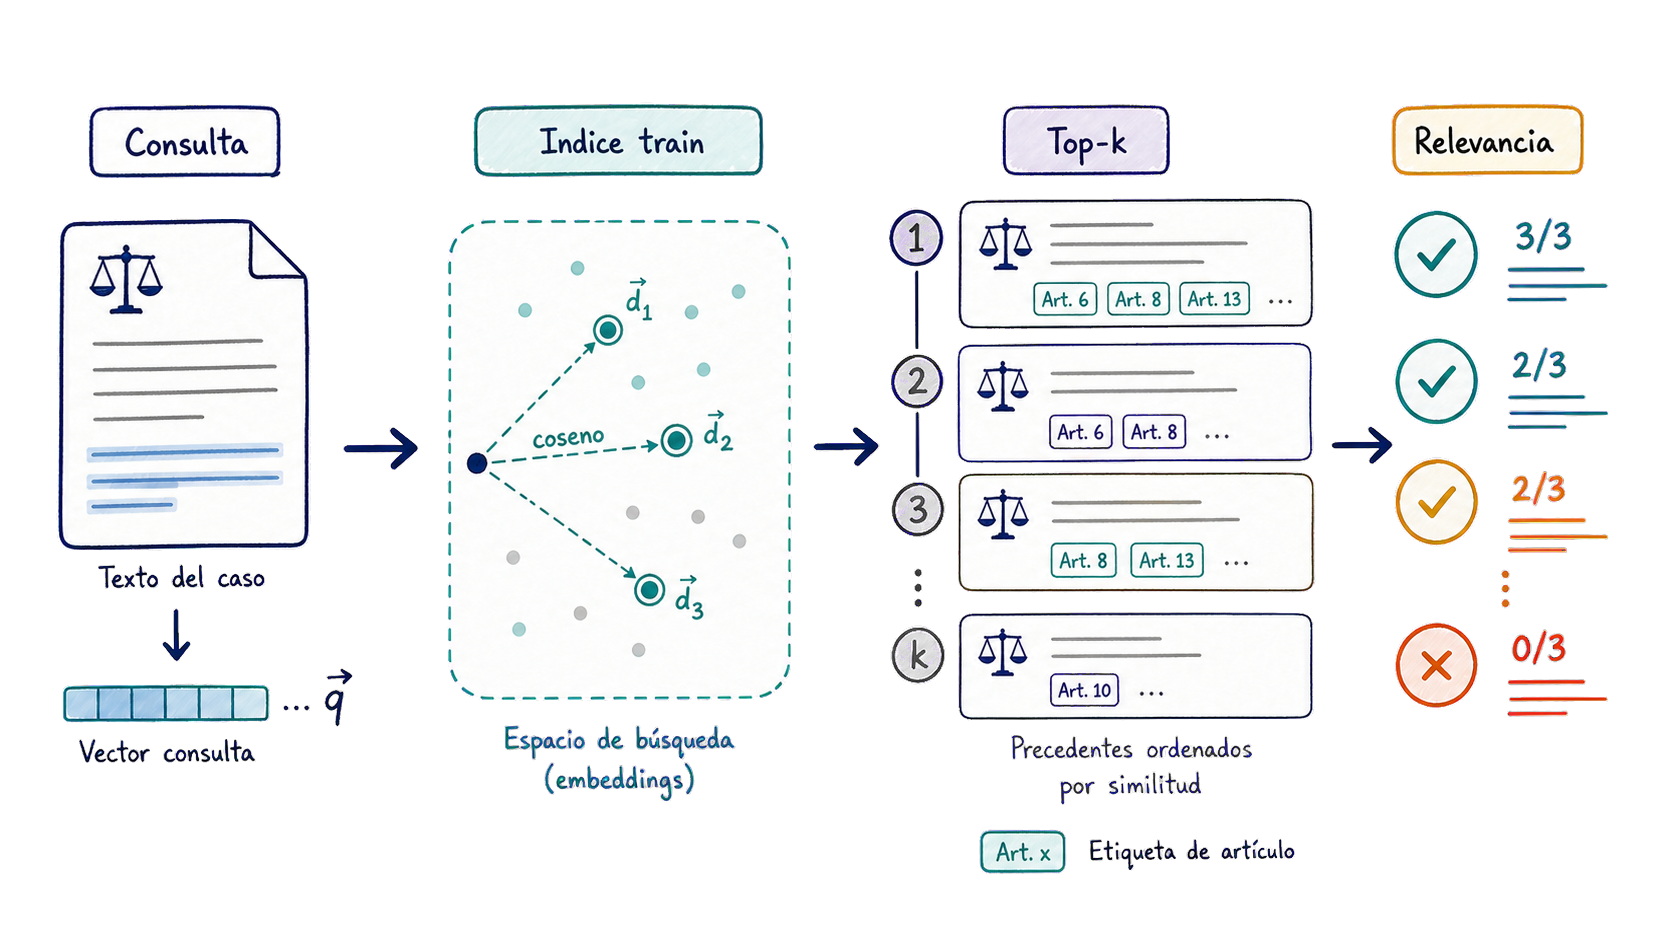
\includegraphics[width=0.92\textwidth]{notebook_03_retrieval_v2.png}
\caption{Esquema del módulo de recuperación de precedentes}
\label{fig_retrieval}
\end{figure}

\subsection{Evaluación}

La evaluación usa una aproximación reproducible. Un caso recuperado se considera relevante si comparte al menos un artículo real con la consulta. Las métricas son Recall@5, Recall@10 y nDCG@10.

Esta definición tiene limitaciones. Dos casos pueden compartir artículo y no ser doctrinalmente parecidos. También pueden ser parecidos y no compartir exactamente la misma etiqueta. Aun así, la definición permite evaluar el ranking sin intervención experta.

\section{Explicabilidad, cambio entre particiones y errores}
\label{sec_auditoria}

\subsection{Explicabilidad global}

En el modelo lineal, cada término tiene un peso por artículo. Un peso positivo alto indica que la presencia del término aumenta el score de esa etiqueta. Un peso negativo indica el efecto contrario. Esto permite construir tablas de términos influyentes.

Por ejemplo, términos relacionados con detención tienden a influir en el artículo 5. Términos relacionados con audiencias y procedimientos tienden a influir en el artículo 6. Términos relacionados con expresión, publicaciones o prensa pueden influir en el artículo 10.

Estas asociaciones son razonables, pero deben interpretarse con cautela. El modelo no entiende el contexto jurídico completo. Solo usa patrones estadísticos de texto.

\subsection{Explicabilidad local}

LIME permite analizar casos concretos. Para una entrada, perturba partes del texto y observa cómo cambia la predicción. Después ajusta una explicación local que indica qué términos han contribuido más.

\begin{figure}[H]
\centering
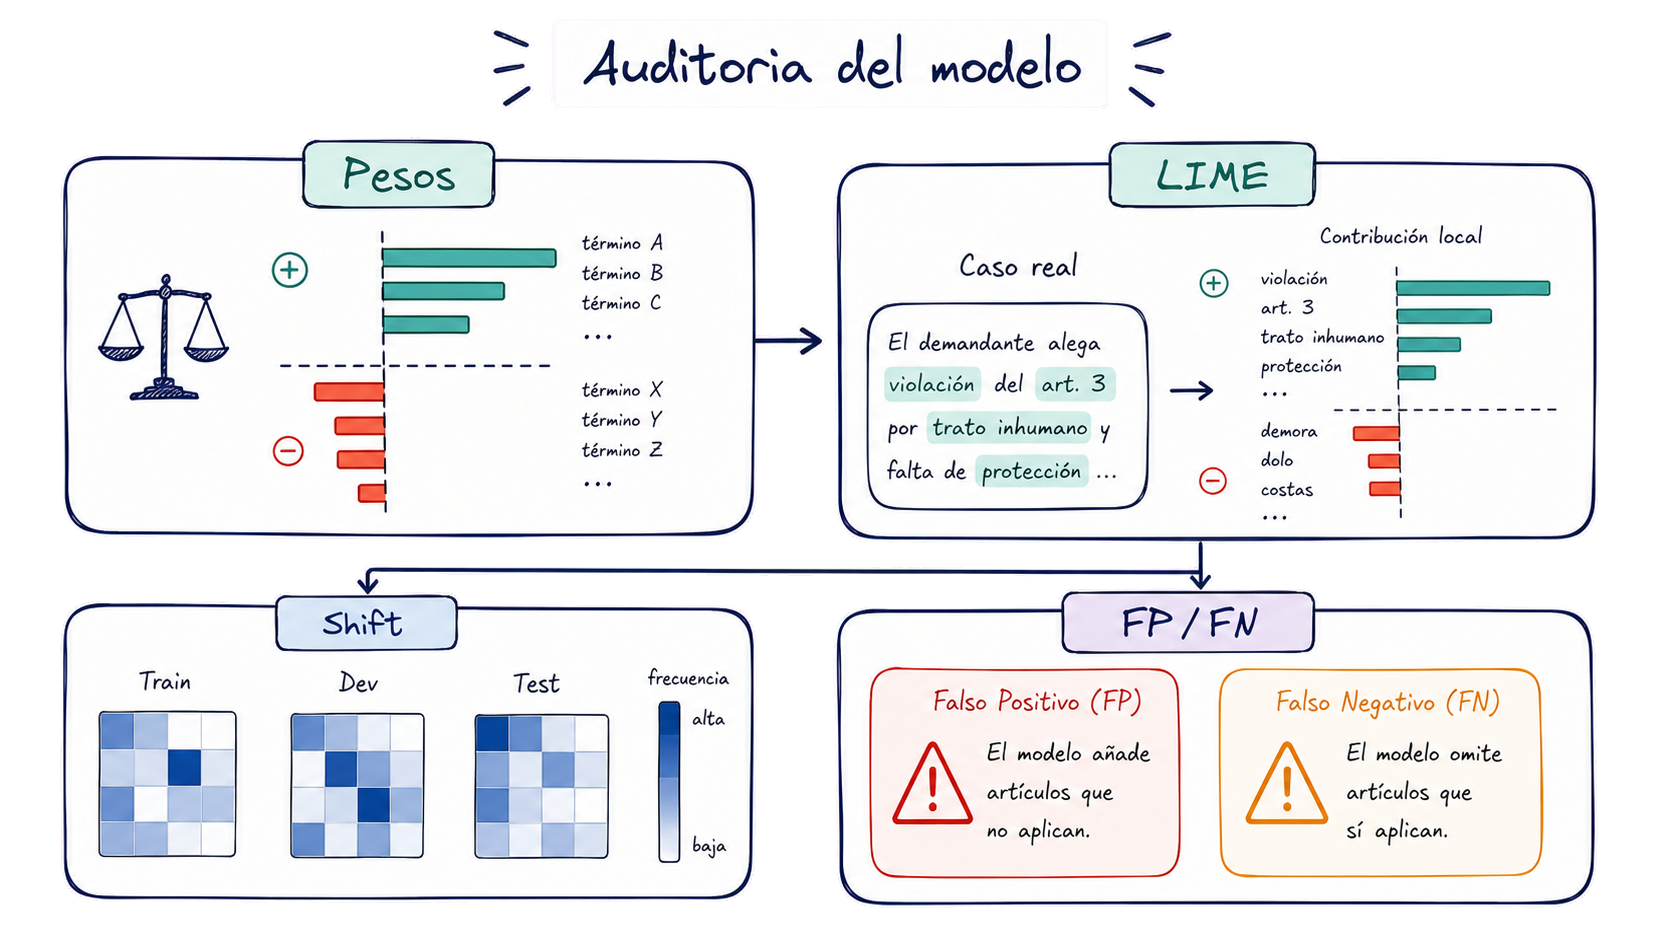
\includegraphics[width=0.92\textwidth]{notebook_04_audit_v2.png}
\caption{Resumen visual de auditoría, explicabilidad y errores}
\label{fig_auditoria}
\end{figure}

El proyecto usa LIME como herramienta de inspección. No se usa como prueba definitiva de causalidad. La explicación local ayuda a detectar si el modelo se apoya en señales plausibles o en palabras accidentales.

\subsection{Cambio entre particiones}

El análisis de cambio compara distribuciones de etiquetas entre train, validation y test. Se usan divergencia Jensen-Shannon, distancia L1 y similitud coseno. También se observan cambios de rendimiento respecto a validation.

Este análisis es importante porque un sistema real no opera siempre sobre datos idénticos a los de entrenamiento. Si cambia la distribución de artículos, el rendimiento puede cambiar. En un dominio jurídico, estos cambios pueden deberse a evolución jurisprudencial, cambios de litigación o diferencias de muestreo.

\subsection{Análisis de errores}

El análisis de errores estudia verdaderos positivos, falsos positivos y falsos negativos por caso. También agrupa patrones frecuentes. Esto permite entender si los fallos suelen ser pequeños, como una etiqueta extra, o más graves, como varias etiquetas perdidas.

La distinción entre FP y FN es clave. Un falso positivo aumenta carga de trabajo. Un falso negativo puede hacer que el usuario no revise un artículo relevante. En una herramienta de apoyo, puede ser preferible aceptar algunos falsos positivos si con ello se reducen falsos negativos en artículos importantes.

\section{Resultados}
\label{sec_resultados}

\subsection{Resultados de clasificación}

La Tabla \ref{tab_cv} recoge la mejor configuración encontrada en validación cruzada para cada modelo. La búsqueda usa solo train y optimiza macro-F1.

\begin{table}[H]
\centering
\caption{Mejores resultados de 5-fold CV sobre train}
\label{tab_cv}
\small
\begin{tabular}{@{}lrrp{0.42\textwidth}@{}}
\toprule
\textbf{Modelo} & \textbf{Macro-F1 CV} & \textbf{Desv.} & \textbf{Mejores hiperparámetros}\\
\midrule
LogReg OVR & 0.726 & 0.036 & \(C=2.0\), \texttt{max\_features}=60000, \texttt{min\_df}=5\\
\rowcolor{bestrow} SVM lineal OVR & \textbf{0.733} & 0.042 & \(C=0.5\), \texttt{max\_features}=30000, \texttt{min\_df}=2\\
SVD + MLP & 0.698 & 0.047 & \texttt{n\_components}=300, capa \((128,)\), \(\alpha=0.0001\), \texttt{max\_features}=30000\\
\bottomrule
\end{tabular}
\end{table}

La Tabla \ref{tab_clasificacion} muestra la comparativa final en test. Estos resultados se calculan una vez fijados los modelos.

\begin{table}[H]
\centering
\caption{Comparativa final de clasificación multietiqueta en test}
\label{tab_clasificacion}
\small
\begin{tabular}{@{}lrrrr@{}}
\toprule
\textbf{Modelo} & \textbf{Casos} & \textbf{Macro-F1} & \textbf{Micro-F1} & \textbf{Hamming loss}\\
\midrule
Baseline frecuente & 1000 & 0.057 & 0.324 & 0.165\\
LogReg OVR & 1000 & 0.736 & 0.760 & 0.069\\
\rowcolor{bestrow} SVM lineal OVR & 1000 & \textbf{0.749} & \textbf{0.777} & \textbf{0.061}\\
SVD + MLP & 1000 & 0.690 & 0.767 & 0.062\\
\bottomrule
\end{tabular}
\end{table}

La SVM lineal obtiene el mejor rendimiento final en test. La regresión logística queda cerca y se conserva como modelo auditado. La MLP no supera a los modelos lineales, aunque ofrece una comparación no lineal útil. El baseline confirma que el problema no se resuelve prediciendo siempre el artículo mayoritario.

La diferencia entre train y test muestra que existe sobreajuste, sobre todo en la SVM. Aun así, el protocolo evita usar test para ajustar decisiones de entrenamiento. Test actúa como evaluación final.

\subsection{Resultados de retrieval}

La Tabla \ref{tab_retrieval} muestra los resultados de recuperación de precedentes.

\begin{table}[H]
\centering
\caption{Resultados de recuperación de precedentes}
\label{tab_retrieval}
\small
\begin{tabular}{@{}llrrrr@{}}
\toprule
\textbf{Método} & \textbf{Split} & \textbf{Consultas} & \textbf{nDCG@10} & \textbf{Recall@5} & \textbf{Recall@10}\\
\midrule
TF-IDF coseno & Validation & 250 & 0.882 & 0.952 & 0.964\\
TF-IDF coseno & Test & 250 & 0.867 & 0.944 & \textbf{0.972}\\
TF-IDF SVD coseno & Validation & 250 & \textbf{0.898} & \textbf{0.960} & 0.964\\
TF-IDF SVD coseno & Test & 250 & 0.876 & 0.940 & 0.956\\
\bottomrule
\end{tabular}
\end{table}

Los resultados indican que el ranking suele recuperar casos con artículos compartidos. Aun así, la evaluación es aproximada. Una revisión experta sería necesaria para validar si esos casos son buenos precedentes en sentido jurídico.

\subsection{Resultados de explicabilidad}

El análisis XAI genera términos globales para diez etiquetas y cinco explicaciones locales. La Tabla \ref{tab_xai} resume los artefactos.

\begin{table}[H]
\centering
\caption{Resumen de explicabilidad}
\label{tab_xai}
\small
\begin{tabular}{@{}rrrr@{}}
\toprule
\textbf{Etiquetas globales} & \textbf{Casos locales} & \textbf{Peso medio absoluto} & \textbf{Probabilidad positiva media}\\
\midrule
10 & 5 & 2.265 & 0.816\\
\bottomrule
\end{tabular}
\end{table}

Los términos globales son coherentes con muchas etiquetas. Por ejemplo, aparecen señales relacionadas con muerte, prisión, audiencia, tribunal o recursos en artículos donde esas palabras son plausibles. Esta coherencia aporta confianza parcial, aunque no elimina el riesgo de correlaciones superficiales.

\subsection{Caso práctico de auditoría local}

El notebook de XAI genera una explicación local para el caso \texttt{ecthr\_task\_b\_test\_000000}. El texto tiene 4774 tokens. El artículo real incluye el artículo 10. El modelo auditado asigna a este artículo una probabilidad positiva de 0.960.

La explicación local muestra términos como \textit{journalist}, \textit{broadcasting}, \textit{journalists} y \textit{press}. Estos términos son coherentes con el artículo 10, que se relaciona con libertad de expresión. Una prueba adicional elimina el término \textit{journalist} y reduce el score de 0.960 a 0.945.

Este ejemplo no demuestra que el artículo esté jurídicamente bien aplicado. Tampoco sustituye una lectura experta. Sirve para ver si la predicción se apoya en señales comprensibles y para facilitar una auditoría local.

\subsection{Cambio entre particiones}

La Tabla \ref{tab_drift} resume el cambio de distribución de etiquetas y rendimiento.

\begin{table}[H]
\centering
\caption{Cambio de distribución respecto a train y cambio de rendimiento respecto a validation}
\label{tab_drift}
\small
\begin{tabular}{@{}lrrrrrr@{}}
\toprule
\textbf{Split} & \textbf{JS} & \textbf{L1} & \textbf{Coseno} & \(\Delta\)\textbf{Macro-F1} & \(\Delta\)\textbf{Micro-F1} & \(\Delta\)\textbf{Hamming}\\
\midrule
Validation & 0.017 & 0.278 & 0.959 & 0.000 & 0.000 & 0.000\\
Test & 0.026 & 0.320 & 0.951 & 0.006 & -0.015 & 0.005\\
\bottomrule
\end{tabular}
\end{table}

El cambio no es extremo, pero existe. Test se aleja más de train que validation. La macro-F1 mejora ligeramente en test, pero micro-F1 baja y Hamming loss aumenta. Esto sugiere que el rendimiento debe vigilarse por varias métricas.

\subsection{Patrones de error}

La Tabla \ref{tab_errores} muestra los patrones más frecuentes en test.

\begin{table}[H]
\centering
\caption{Patrones de error más frecuentes en test}
\label{tab_errores}
\small
\begin{tabular}{@{}rrr@{}}
\toprule
\textbf{Falsos positivos} & \textbf{Falsos negativos} & \textbf{Casos}\\
\midrule
0 & 0 & 491\\
1 & 0 & 189\\
0 & 1 & 170\\
1 & 1 & 65\\
0 & 2 & 36\\
2 & 0 & 25\\
\bottomrule
\end{tabular}
\end{table}

La tabla se lee por caso, no por artículo. Un falso positivo es un artículo que el modelo añade aunque no aparezca en la etiqueta real. Un falso negativo es un artículo real que el modelo no detecta. Por ejemplo, 491 casos no tienen ningún error. En 189 casos el modelo añade un artículo de más, pero no omite ninguno. En 170 casos ocurre lo contrario. No añade artículos incorrectos, pero deja sin detectar un artículo real. Esto muestra que muchos fallos son pequeños, aunque los falsos negativos siguen siendo importantes porque pueden ocultar artículos relevantes.

\section{Validación y reproducibilidad}
\label{sec_validacion}

\subsection{Protocolo de validación}

El proyecto usa las particiones oficiales del benchmark. Train se usa para seleccionar hiperparámetros con \texttt{GridSearchCV} y validación cruzada de 5 folds. El vectorizador TF-IDF forma parte del \texttt{Pipeline}, por lo que se ajusta dentro de cada fold solo con los datos correspondientes.

Tras la búsqueda, el mejor estimador se reentrena con todo train mediante \texttt{refit=True}. Test se usa una sola vez para la evaluación final. No se usa test para ajustar hiperparámetros, umbrales, arquitectura ni decisiones de entrenamiento.

Validation queda como partición informativa para análisis auxiliares. No decide el modelo final ni los hiperparámetros principales.

\subsection{Métricas}

Se usan métricas adecuadas para clasificación multietiqueta. Macro-F1 calcula F1 por etiqueta y después promedia. Da más visibilidad a etiquetas raras. Micro-F1 agrega verdaderos positivos, falsos positivos y falsos negativos antes de calcular F1. Refleja mejor el rendimiento global. Hamming loss mide la proporción de decisiones etiqueta caso incorrectas.

Para retrieval se usan Recall@5, Recall@10 y nDCG@10. Recall@k mide si aparecen relevantes entre los primeros resultados. nDCG@10 también tiene en cuenta la posición del resultado relevante dentro del ranking.

\subsection{Semillas y artefactos}

El proyecto fija semilla 42 en Python y NumPy. Los artefactos se guardan en carpetas separadas. Las predicciones se almacenan en SQLite junto a scores y etiquetas reales. Esta organización permite reproducir tablas y revisar errores concretos.

La memoria se ha preparado a partir de los notebooks ejecutados y de los artefactos guardados. Los CSV de métricas, las predicciones, los mejores hiperparámetros y los modelos finales permiten revisar los resultados sin rehacer el análisis manualmente.

\section{Discusión crítica}
\label{sec_discusion}

\subsection{Interpretación de los resultados}

El sistema obtiene resultados razonables para una solución clásica y transparente. El modelo es capaz de capturar señales textuales asociadas a artículos. El retrieval recupera casos que comparten etiquetas con alta frecuencia. Las explicaciones globales muestran términos que en muchos casos son jurídicamente plausibles.

Sin embargo, estas cifras no justifican automatizar decisiones. El modelo trabaja con texto y etiquetas del benchmark. No evalúa pruebas, no interpreta normas completas y no razona como un jurista. Su valor está en priorizar revisión.

\subsection{Riesgos de falsos positivos y falsos negativos}

Los falsos positivos pueden inducir revisión innecesaria. También pueden generar anclaje. Si el sistema sugiere un artículo, el usuario puede prestarle demasiada atención aunque sea irrelevante.

Los falsos negativos son más delicados. Si el sistema no sugiere un artículo, el usuario podría no revisarlo. En una herramienta real se podría estudiar un ajuste de umbrales según coste de error. Ese ajuste tendría que hacerse sin usar test como conjunto de decisión.

\subsection{Riesgos del retrieval}

El retrieval puede ser útil para encontrar casos parecidos, pero también puede reforzar analogías débiles. La similitud coseno sobre TF-IDF se basa en vocabulario compartido. Dos casos pueden usar palabras parecidas y tener problemas jurídicos distintos. También puede ocurrir lo contrario. Dos casos pueden ser doctrinalmente cercanos y usar vocabulario distinto.

Por eso los precedentes recuperados deben entenderse como una lista de lectura inicial, no como una selección definitiva.

\subsection{Límites de la explicabilidad}

Los coeficientes y LIME ayudan a inspeccionar el modelo. Aun así, una explicación técnica no es una justificación jurídica. Un término puede ser predictivo porque aparece en muchos casos de un artículo, pero la relevancia legal depende del contexto.

Además, LIME aproxima localmente el comportamiento del modelo. Esa aproximación puede variar según perturbaciones y parámetros. Por tanto, sus resultados deben usarse como apoyo a la auditoría, no como explicación completa.

\subsection{Privacidad y despliegue}

El proyecto usa datos públicos. Por eso no se implementan técnicas como aprendizaje federado o privacidad diferencial. En un despliegue real, el escenario sería distinto. Los expedientes podrían contener información sensible. Sería necesario controlar acceso, anonimizar datos, registrar consultas y definir si el procesamiento ocurre localmente o en una infraestructura aprobada.

También sería necesario comunicar al usuario el alcance del sistema. La interfaz debería mostrar incertidumbre, artículos alternativos y advertencias sobre supervisión humana.

\section{Limitaciones}
\label{sec_limitaciones}

El proyecto tiene varias limitaciones.

\begin{itemize}
    \item TF-IDF no captura semántica profunda ni relaciones jurídicas complejas.
    \item Los modelos lineales son interpretables, pero pueden perder matices contextuales.
    \item La evaluación de retrieval usa artículos compartidos como proxy de relevancia.
    \item No hay evaluación cualitativa por expertos jurídicos.
    \item El análisis de cambio entre particiones no equivale a deriva temporal estricta.
    \item Las explicaciones no prueban causalidad.
    \item El dataset público no representa todos los problemas de privacidad de un uso real.
    \item Los resultados dependen de las etiquetas del benchmark y de su calidad.
\end{itemize}

Estas limitaciones no invalidan el proyecto. Delimitan su alcance y ayudan a interpretar correctamente sus resultados.

\section{Trabajo futuro}
\label{sec_futuro}

La primera mejora sería evaluar los precedentes recuperados con expertos jurídicos. Esto permitiría saber si los casos devueltos son útiles más allá de compartir artículos.

La segunda mejora sería estudiar calibración de probabilidades. Un sistema de apoyo debería comunicar incertidumbre de forma clara. La calibración permitiría interpretar mejor los scores.

La tercera mejora sería estudiar umbrales según coste de error. Algunos artículos podrían requerir alta sensibilidad. Otros podrían priorizar precisión. Esta mejora tendría que evaluarse con validación interna o con un nuevo conjunto de desarrollo, nunca usando test para decidir.

La cuarta mejora sería comparar de forma controlada con modelos jurídicos contextualizados, como variantes de BERT adaptadas al dominio legal. También se podrían probar redes neuronales más grandes. Sin embargo, aumentar complejidad puede elevar el coste y el riesgo de sobreajuste sin garantizar mejora. La comparación debería mantener la selección de hiperparámetros sin usar test.

La quinta mejora sería incorporar una estrategia real de monitorización. Esto incluiría drift, errores por etiqueta, distribución de consultas y alertas de degradación.

La sexta mejora sería diseñar un protocolo de privacidad para uso con datos sensibles. Este protocolo debería incluir anonimización, control de acceso, auditoría y límites de uso.

\section{Conclusiones}
\label{sec_conclusiones}

Este trabajo ha desarrollado un sistema completo de apoyo al análisis inicial de casos del TEDH. El sistema combina clasificación multietiqueta, recuperación de precedentes, explicabilidad y análisis de errores. La solución se ha diseñado para ser reproducible, auditable y fácil de explicar.

La principal aportación técnica es el pipeline. Los datos se estructuran en SQLite. Los textos se vectorizan con TF-IDF dentro de un \texttt{Pipeline}. Los artículos se predicen con modelos One-vs-Rest. Los hiperparámetros se seleccionan con \texttt{GridSearchCV} y 5 folds usando solo train. Los precedentes se recuperan por similitud. Las predicciones se auditan con coeficientes, LIME y análisis de errores.

Los resultados muestran utilidad parcial. En test, el modelo final por rendimiento es la SVM lineal, con macro-F1 de 0.749 y micro-F1 de 0.777. La regresión logística auditada obtiene macro-F1 de 0.736 y micro-F1 de 0.760. El retrieval alcanza Recall@10 de 0.972 con TF-IDF coseno. Estas cifras indican que el sistema puede ayudar a priorizar lectura, pero no puede reemplazar criterio jurídico.

La conclusión más importante es que el valor de un sistema de ML en derecho no depende solo de una métrica. También depende de su alcance, interpretabilidad, control de errores, robustez y forma de comunicación al usuario. En este proyecto, esos elementos forman parte central de la solución.

\appendix

\section{Anexo A. Archivos principales}
\label{anexo_archivos}

\begin{table}[H]
\centering
\caption{Papel de los archivos más importantes}
\small
\begin{tabular}{@{}p{0.31\textwidth}p{0.61\textwidth}@{}}
\toprule
\textbf{Archivo} & \textbf{Función}\\
\midrule
\texttt{README.md} & Documenta objetivo, instalación, ejecución, resultados, artefactos y limitaciones.\\
\texttt{schema.sql} & Define la base SQLite usada como estructura común.\\
\texttt{project\_utils.py} & Contiene rutas, constantes, carga de datos, creación de matrices y métricas.\\
\texttt{00\_ingesta...ipynb} & Crea la base relacional desde LexGLUE.\\
\texttt{01\_EDA.ipynb} & Analiza calidad, splits, longitudes, frecuencias y coocurrencias.\\
\texttt{02\_modelado...ipynb} & Entrena modelos con GridSearchCV, evalúa test y guarda predicciones.\\
\texttt{03\_retrieval...ipynb} & Construye y evalúa índices de precedentes.\\
\texttt{04\_xai...ipynb} & Audita explicabilidad, cambio entre particiones y errores.\\
\texttt{05\_guion...ipynb} & Revisa artefactos y organiza evidencias para defensa.\\
\bottomrule
\end{tabular}
\end{table}

\section{Anexo B. Reproducción}
\label{anexo_reproduccion}

Para reproducir el proyecto en un entorno limpio se recomienda crear un entorno virtual, instalar dependencias y ejecutar los notebooks en orden.

\begin{lstlisting}[language=bash]
python -m venv .venv
.venv\Scripts\activate
pip install -r requirements.txt
\end{lstlisting}

Después se ejecutan los notebooks desde la raíz del proyecto.

\begin{lstlisting}[language=bash]
jupyter nbconvert --to notebook --execute 00_ingesta_y_esquema_relacional.ipynb --inplace
jupyter nbconvert --to notebook --execute 01_EDA.ipynb --inplace
jupyter nbconvert --to notebook --execute 02_modelado_multilabel.ipynb --inplace
jupyter nbconvert --to notebook --execute 03_retrieval_de_precedentes.ipynb --inplace
jupyter nbconvert --to notebook --execute 04_xai_drift_y_errores.ipynb --inplace
jupyter nbconvert --to notebook --execute 05_guion_informe_y_defensa.ipynb --inplace
\end{lstlisting}

\section{Anexo C. Referencias}
\label{anexo_referencias}

\begin{thebibliography}{9}

\bibitem{chalkidis2022lexglue}
Chalkidis, I., Jana, A., Hartung, D., Bommarito, M., Androutsopoulos, I., Katz, D. M. y Aletras, N.
\newblock LexGLUE. A benchmark dataset for legal language understanding in English.
\newblock \textit{Proceedings of the 60th Annual Meeting of the Association for Computational Linguistics}, 2022.

\bibitem{chalkidis2020legalbert}
Chalkidis, I., Fergadiotis, M., Malakasiotis, P., Aletras, N. y Androutsopoulos, I.
\newblock LEGAL-BERT. The muppets straight out of law school.
\newblock \textit{Findings of EMNLP}, 2020.

\bibitem{aletras2016predicting}
Aletras, N., Tsarapatsanis, D., Preoţiuc-Pietro, D. y Lampos, V.
\newblock Predicting judicial decisions of the European Court of Human Rights from text.
\newblock \textit{PeerJ Computer Science}, 2016.

\bibitem{ribeiro2016lime}
Ribeiro, M. T., Singh, S. y Guestrin, C.
\newblock Why should I trust you. Explaining the predictions of any classifier.
\newblock \textit{Proceedings of KDD}, 2016.

\bibitem{gama2014survey}
Gama, J., Zliobaite, I., Bifet, A., Pechenizkiy, M. y Bouchachia, A.
\newblock A survey on concept drift adaptation.
\newblock \textit{ACM Computing Surveys}, 2014.

\bibitem{moreno2012datasetshift}
Moreno-Torres, J. G., Raeder, T., Alaiz-Rodriguez, R., Chawla, N. V. y Herrera, F.
\newblock A unifying view on dataset shift in classification.
\newblock \textit{Pattern Recognition}, 2012.

\end{thebibliography}

\end{document}
